
\section{Dynamical quantum $SU(2)$}

\subsection{Dynamical quantum $SU(2)$ from the Podle\'{s} graph}

Let us now consider the particular case of the Podle\'{s} graph of Example \ref{ExaGraphPod}. We assume in the following that $x\in \lbrack 0,\frac{1}{2}\rbrack$.

Let us denote

\[w_+(k) = w(k,k+1),\]\[w_-(k)  = w(k,k-1) = w_+(k-1)^{-1}.\] 

Let $A_x = A(\Gamma_x)$ be the total $^*$-algebra of the associated partial compact quantum group. Using Theorem \ref{TheoGenRel}, we have the following presentation of $A_x$. Let $B$ be the $^*$-algebra of finite support functions on $\Z\times \Z$, whose Dirac functions we write as $\UnitC{k}{l}$. Let $s_q = \frac{1}{2}(1+\sgn(q))$. Then $A_x$ is generated by a copy of $B$ and elements \[(u_{\epsilon,\nu})_{k,l} = u_{(k,k+\epsilon),(l,l+\nu)}\] for $\epsilon,\nu\in \{-1,1\}=\{-,+\}$ and $k,l\in \Z$ with defining relations \begin{eqnarray*} \sum_{\mu\in \{\pm\}} (u_{\mu,\epsilon})_{m-\mu,k}^* (u_{\mu,\nu})_{m-\mu,l}&=& \delta_{k,l} \delta_{\epsilon,\nu} \UnitC{m}{k+\epsilon},\\ \sum_{\mu\in \{\pm\}} (u_{\epsilon,\mu})_{k,m} (u_{\nu,\mu})_{l,m}^* &=& \delta_{\epsilon,\nu}\delta_{k,l} \UnitC{k}{m}\\ (u_{\epsilon,\nu})_{k,l}^* &=& (\epsilon\nu)^{s_q} \left(\frac{w_{\nu}(l)}{w_{\epsilon}(k)}\right)^{1/2} (u_{-\epsilon,-\nu})_{k+\epsilon,l+\nu}.\end{eqnarray*} The element $(u_{\epsilon,\nu})_{k,l}$ lives inside the component $\Gr{(A_x)}{k}{k+\epsilon}{l}{l+\nu}$.

Consider now $M(A_x)$, the multiplier algebra of $A_x$. We can form in $M(A_x)$ the elements $u_{\epsilon,\nu} = \sum_{k,l} (u_{\epsilon,\nu})_{k,l}$. Then $u=(u_{\epsilon,\nu})$ is a unitary 2$\times$2 matrix. Moreover, \begin{equation}\label{EqAdju}u_{\epsilon,\nu}^* = (\epsilon\nu)^{s_q} u_{-\epsilon,-\nu}\frac{w_{\nu}^{1/2}(\rho)}{w_{\epsilon}^{1/2}(\lambda)} ,\end{equation} where $w_{\pm}^{1/2}(k) = w_{\pm}(k)^{1/2}$ and where for a function $f$ on $\Z$ we write $f(\lambda)(k,l) = f(k)$, $f(\rho)(k,l) = f(l)$. In the following, we then also use the notation $f(\lambda,\rho)$ for a function $f$ on $\Z\times \Z$ interpreted as an element of $M(A)$, and for example $f(\lambda+1,\rho)$ corresponds to the function $(k,l)\mapsto f(k+1,l)$. We then have the following commutation relations between functions on $\Z\times \Z$ and the entries of $u$: \begin{equation}\label{EqGradu} f(\lambda,\rho)u_{\epsilon,\nu} = u_{\epsilon,\nu}f(\lambda-\epsilon,\rho-\nu).\end{equation}

%The relations for the adjoint further imply that \begin{eqnarray*}u_{kl}^{+-} &=&\frac{E(l,l-1)}{E(k,k+1)}(u_{k+1,l-1}^{-+})^*,\\  u_{kl}^{++}&=& \frac{E(l,l+1)}{E(k,k+1)}(u_{k+1,l+1}^{--})^* .\end{eqnarray*}


%\begin{eqnarray*} u_{++} &=& \frac{w_+(\rho)^{1/2}}{w_+(\lambda)^{1/2}}u_{--}^*,\\u_{+-}&=& (-1)^{s_q}  \frac{w_-^{1/2}(\rho)}{w_+^{1/2}(\lambda)}u_{-+}^*.  \\ 
%\end{eqnarray*}

Let us write \[F(k) = |q|^{-1}w_+(k) =  |q|^{-1}\frac{|q|^{x+k+1}+|q|^{-x-k-1}}{|q|^{x+k}+|q|^{-x-k}},\] and further put\[\alpha = \frac{F^{1/2}(\rho-1)}{F^{1/2}(\lambda-1)}u_{--},\qquad \beta = \frac{1}{F^{1/2}(\lambda-1)}u_{-+}.\] Then the unitarity of $(u_{\epsilon,\nu})_{\epsilon,\nu}$ together with \eqref{EqAdju} and \eqref{EqGradu} are equivalent to the commutation relations \begin{equation}\label{EqqCom} \alpha \beta = qF(\rho-1)\beta\alpha \qquad \alpha\beta^* = qF(\lambda)\beta^*\alpha\end{equation} \begin{equation}\label{EqDet} \alpha\alpha^* +F(\lambda)\beta^*\beta = 1,\qquad \alpha^*\alpha+q^{-2}F(\rho-1)^{-1}\beta^*\beta = 1,\end{equation}\begin{equation*} F(\rho-1)^{-1}\alpha\alpha^* +\beta\beta^* = F(\lambda-1)^{-1},\qquad  F(\lambda)\alpha^*\alpha +q^{-2}\beta\beta^* = F(\rho),\end{equation*} \begin{equation}\label{EqGrad} f(\lambda)g(\rho)\alpha =
\alpha f(\lambda+1)g(\rho+1),\qquad f(\lambda)g(\rho)\beta = \beta f(\lambda+1)g(\rho-1).\end{equation}%layout might be nicer

These are precisely the commutation relations for the dynamical quantum $SU(2)$-group as in \cite[Definition 2.6]{KoR1}, except that the precise value of $F$ has been changed by a shift in the parameter domain by a complex constant. Clearly, by Theorem \ref{TheoGenRel} the (total) coproduct on $A_x$ also agrees with the one on the dynamical quantum $SU(2)$-group, namely \begin{eqnarray*} \Delta(\alpha) &=& \Delta(1) (\alpha\otimes \alpha - q^{-1}\beta\otimes \beta^*),\\ \Delta(\beta) &=& \Delta(1)(\beta\otimes \alpha^* +\alpha\otimes \beta)\end{eqnarray*} where $\Delta(1) = \sum_{k\in \Z} \rho_k\otimes \lambda_k$.

\subsection{Representation theory of the function algebra of dynamical quantum $SU(2)$}

%Then we study the regular representation. We then show explicitly that the quantum groupoid is amenable in the sense that the universal C$^*$-envelope coincides with the regular representation.

In this section we classify the irreducible $^*$-representations of $A_x$. The parametrisation will hinge on the classification of what we call irreducible $(x,c)$-adapted sets, which we will now discuss. In the following, we fix $0<|q|<1$.

\begin{Def}\label{DefAdapt} Let $x\in \lbrack 0,\frac{1}{2}\rbrack$, and let $c\in\R$. For $\epsilon \in \{\pm\}$, an integer $m\in \Z$ will be called \emph{$(x,c)_{\epsilon}$-adapted} if \begin{equation}\label{EqAd+}c \leq |q|^{2x+m-\epsilon}+|q|^{-2x-m+\epsilon},\end{equation} and \emph{strictly} $(x,c)_{\epsilon}$-adapted if this holds strictly. An integer is called \emph{$(x,c)$-adapted} if it is both $(x,c)_+$ and $(x,c)_-$-adapted. 

A set of integers $Z$ is called an  \emph{$(x,c)$-set} if the following conditions hold: \begin{itemize} 
\item[$\bullet$] $Z$ is not empty.
\item[$\bullet$] $Z$ consists of $(x,c)$-adapted points.
\item[$\bullet$] If $m\in Z$ is strictly $(x,c)_{\epsilon}$-adapted, then $m-2\epsilon$ is in $Z$.
\end{itemize}
An $(x,c)$-set $Z$ is called \emph{even} (resp. \emph{odd}) if $Z\subseteq 2\Z$ (resp. $Z\subseteq 2\Z+1$).

An $(x,c)$-set is called \emph{irreducible} if it can not be written as the union of two disjoint $(x,c)$-sets.
\end{Def}


We aim to classify irreducible $(x,c)$-sets. We start of with the following lemma.

\begin{Lem} Let $c\in\R$ and $x\in \lbrack 0,\frac{1}{2}\rbrack$.
\begin{enumerate} \item Any irreducible $(x,c)$-set is either even or odd.
\item $Z$ is an irreducible $(x,c)$-set if and only if $-Z-1$ is an irreducible $(\frac{1}{2}-x,c)$-set.
\end{enumerate}
\end{Lem}

\begin{proof} Immediate.
\end{proof}

Hence it suffices to classify even irreducible $(x,c)$-sets. This is achieved in the following proposition. (We use the convention $\N = \{0,1,2,\ldots\}$ and $\N_0=\{1,2,\ldots\}$).

\begin{Prop}\label{PropClass1D} Let $c\in \R$ and $x\in \lbrack 0,\frac{1}{2}\rbrack$.  
\begin{itemize}
\item[$\bullet$] If $c< |q|^{2x-1}+|q|^{-2x+1}$, then $2\Z$ is an irreducible $(x,c)$-set.
\item[$\bullet$] If $c\geq |q|^{2x-1}+|q|^{-2x+1}$, write $c=|q|^y+|q|^{-y}$ for some unique $y\geq 1-2x$. 
\begin{itemize}\item[$*$] Assume $x=0$.
\begin{itemize}\item[$\circ$] If $y=1$, then $-2\N_0$, $\{0\}$ and $2\N_0$ are irreducible $(x,c)$-sets.
\item[$\circ$] If $y\in 2\N_0+1$, then $y+1+2\N$ and $-y-1-2\N$ are irreducible $(x,c)$-sets.
\end{itemize}
\item[$*$] Assume $x\in (0,\frac{1}{2})$. Assume $y$ is of the form $y=|2x+M-1|$, where $M$ is a (uniquely determined) even integer. 
\begin{itemize}\item[$\circ$] If $M>0$, then $M+2\N$ is an irreducible $(x,c)$-set. 
\item[$\circ$] If $M<0$, then $M-2\N_0$ is an irreducible $(x,c)$-set. 
\item[$\circ$] If $M=0$, then $2\N$ and $-2\N_0$ are irreducible $(x,c)$-sets.
\end{itemize}
\item[$*$] Assume $x=\frac{1}{2}$.
\begin{itemize}\item[$\circ$] If $y\in 2\N$, then $y+2\N$ and $-y-2\N_0$ are irreducible $(x,c)$-sets.
\end{itemize}
\end{itemize}
\end{itemize}
The above $(x,c)$-sets exhaust all possible even irreducible $(x,c)$-sets.
\end{Prop} 
\begin{proof}
Clearly \[\min \{|q|^{2x+m-\epsilon}+|q|^{-2x-m+\epsilon}\mid m\in 2\Z,\epsilon\in \{-1,1\}\} = |q|^{2x-1}+|q|^{-2x+1}.\] Hence if $c< |q|^{2x-1}+|q|^{-2x+1}$, all $m\in 2\Z$ are strictly $(x,c)_{\epsilon}$-adapted for any $\epsilon\in \{-1,1\}$, and we deduce that $2\Z$ is the only irreducible $(x,c)$-set.

If $c\geq |q|^{2x-1}+|q|^{-2x+1}$, we can write $c=|q|^y+|q|^{-y}$ for a uniquely determined $y\geq 1-2x$, and then we see $m$ is $(x,c)_{\epsilon}$-adapted if and only if \[ y \leq |2x+m-\epsilon|.\]

If $y=1-2x$, we can still conclude that $2\Z$ is an $(x,c)$-set, but it will no longer be irreducible. If $m\in 2\N_0$ and $x\neq 0$, then it is strictly $(x,c)_{\epsilon}$-adapted for $\epsilon\in \{-,+\}$, hence if an irreducible $(x,c)$-set contains a strictly positive even integer, it contains $2\N$. Since $m=0$ is $(x,c)$-adapted but not strictly $(x,c)_+$-adapted, we conclude that $2\N$ is an irreducible $(x,c)$-set. In case $x=0$ however, $m=2$ is not strictly $(x,c)_+$-adapted, and we can conclude that in fact $2\N_0$ is an irreducible $(x,c)$-set. The set $\{0\}$ then is an irreducible $(x,c)$-set by itself. Considering again a general $x$, we similarly see that if an irreducible $(x,c)$-set contains an even integer $<2$, then it contains $-2\N_0$. Hence $-2\N_0$ is an irreducible $(x,c)$-set. Hence for $x\neq 0$,  $2\N$ and $-2\N_0$ exhaust the irreducible $(x,c)$-sets, while for $x=0$ we have the three sets $2\N_0,\{0\}$ and $-2\N_0$.

If $y>1-2x$, it is clear that an $(x,c)$-set exists if and only if the equation $y=|2x+m-1|$ admits a solution in $2\Z$. 

Let us first assume that $x\in (0,\frac{1}{2})$. Then this solution is unique, say $y=|2x+M-1|$ with $M\in 2\Z$. 

Assume first that $M>0$. Then any even $m< 0$ which is $(x,c)_-$-adapted is strictly $(x,c)_{-}$-adapted. It follows that if an $(x,c)$-set contains a strictly negative integer, it contains $m=0$. But then $m=0$ is $(x,c)_+$-adapted, which leads to the contradictory statement $x\leq0$. Hence any $(x,c)$-set necessarily lies in $2\N_0$. It is then easily seen that the only $(x,c)$-set is $M+2\N$, which is then necessarily irreducible.

Assume now that $M\leq 0$. From the condition $y>1-2x$, we may in fact assume $M<0$. Then as above, we conclude that if an $(x,c)$-set contains a strictly positive even integer, it contains $m=0$, which is not $(x,c)_-$-adapted. It then follows that $M-2\N_0$ is the only irreducible $(x,c)$-set.

Let us now assume that $x=0$. Then we may assume $y=M+1$ with $M\in 2\N_0$. Then $m>0$ is $(x,c)_+$-adapted if and only if $m\geq M+2$, and it is strictly so if and only if $m>M+2$. As $m=M+2$ is $(x,c)$-adapted, it follows that $M+2\N_0$ is an irreducible $(x,c)$-set, and the only one which intersects the strictly positive integers non-trivially. On the other hand, an $m<0$ is $(x,c)_-$-adapted if and only if $m\leq -M-2$, and strictly so if and only if $m<-M-2$. As $m=-M-2$ is $(x,c)$-adapted, it follows that $-M-2\N_0$ is an irreducible $(x,c)$-set, and the only one which intersects the strictly negative integers non-trivially. Finally, since we have assumed $M>0$, the integer $m=0$ is never $(x,c)$-adapted.

Finally, let us assume that $x=\frac{1}{2}$. Then we may assume $y=M$ with $M\in 2\N_0$. By a similar reasoning as in the case $x=0$, we conclude that the only irreducible $(x,c)$-sets are $M+2\N$ and $-M-2\N_0$.
\end{proof} 

Let us now return to the representation theory of the $^*$-algebra $A_x$.

Let $\pi$ be any (necessarily bounded) non-degenerate $^*$-representation of $A_x$ on a Hilbert space $\Hsp_{\pi}$. Then \[\Hsp_{\pi} = \oplus \Hsp^{m}_{n},\qquad \Hsp^{m}_{n} = \pi(\UnitC{m}{n})\Hsp.\] Write \[V_{\pi} =  \textrm{the (non-closed) linear span of all }\Hsp^{m}_{n}.\] Then $\pi(A_x)V_{\pi} = V_{\pi}$. It follows that one can extend $\pi$ to a map \[\pi: M(A_x) \rightarrow \End_{\adj}(V_{\pi}),\] where $\End_{\adj}(V_{\pi})$ denotes the $^*$-algebra of adjointable operators on the pre-Hilbert space $V_{\pi}$. As the $u_{\epsilon,\nu}$ form a unitary matrix, we can then in fact make sense of the $\pi(u_{\epsilon,\nu})$ as contractions on $\Hsp_{\pi}$. Hence the generators $\alpha,\beta$ and their adjoints give rise to endomorphisms $V_{\pi}\rightarrow V_{\pi}$ which are bounded when restricted to any $\Hsp^{m}_{n}$.

We then have the following easy lemma.

\begin{Lem} There is a one-to-one correspondence between\begin{itemize}\item[$\bullet$] non-degenerate $^*$-representations $(\Hsp_{\pi},\pi)$ of $A_x$ on Hilbert spaces, and 
\item[$\bullet$] $\Z^2$-bigraded pre-Hilbert spaces $V_{\pi}$ with norm-complete components and equipped with adjointable maps $\alpha,\beta:V_{\pi}\rightarrow V_{\pi}$ satisfying the commutation relations as in \eqref{EqqCom}, \eqref{EqDet} and \eqref{EqGrad} and with $f(\lambda,\rho)\xi = f(k,l)\xi$ for $f$ a function on $\Z\times \Z$ and $\xi\in V^k_l$.
\end{itemize}
\end{Lem}

\begin{Def} The \emph{Casimir} of $A_x$ is defined to be the following element $\Omega\in M(A_x)$, \[\Omega =q^{\lambda-\rho+1}+q^{\rho-\lambda-1} - \sgn(q)^{\lambda-\rho}q^{-1}(|q|^{x+\lambda+1}+|q|^{-x-\lambda-1})(|q|^{x+\rho-1}+|q|^{-x-\rho+1})\beta^*\beta.\] 
\end{Def}

\begin{Lem} The element $\Omega$ is  self-adjoint central in $M(A_x)$.
\end{Lem}
\begin{proof}
Straightforward, cf. \cite[Lemma 3.3]{KoR1}.
\end{proof}

\begin{Cor}\label{CorCas} If $\pi$ is an irreducible $^*$-representation of $A_x$, there exists $c\in \R$ such that $\pi(\Omega)\xi = c\xi$ for all $\xi \in V_{\pi}$. 
\end{Cor} 
\begin{proof} As $\pi(\Omega)$ is bounded when restricted to any $V^k_l$, this follows immediately from a spectral argument. 
\end{proof} 

The following lemma follows from a straightforward computation, using the relations \eqref{EqDet}.

\begin{Lem}\label{LemAmp} Inside $M(A_x)$, we have the following identities:
\begin{eqnarray*}
\alpha^*\alpha &=& \frac{|q|^{2x+\lambda+\rho+1}+|q|^{-2x-\lambda-\rho-1}+\sgn(q)^{\lambda-\rho+1}\Omega}{(|q|^{x+\lambda+1}+|q|^{-x-\lambda-1})(|q|^{x+\rho}+|q|^{-x-\rho})}\\
\alpha\alpha^* &=& \frac{|q|^{2x+\lambda+\rho-1}+|q|^{-2x-\lambda-\rho+1}+\sgn(q)^{\lambda-\rho-1}\Omega}{(|q|^{x+\lambda}+|q|^{-x-\lambda})(|q|^{x+\rho-1}+|q|^{-x-\rho+1})}\\
\beta^*\beta &=& |q|\frac{|q|^{\lambda-\rho+1}+|q|^{-\lambda+\rho-1}-\sgn(q)^{\lambda-\rho+1}\Omega}{(|q|^{x+\lambda+1}+|q|^{-x-\lambda-1})(|q|^{x+\rho-1}+|q|^{-x-\rho+1})}\\
\beta\beta^* &=&  |q|\frac{|q|^{\lambda-\rho-1}+|q|^{-\lambda+\rho+1}-\sgn(q)^{\lambda-\rho-1}\Omega}{(|q|^{x+\lambda}+|q|^{-x-\lambda})(|q|^{x+\rho}+|q|^{-x-\rho})}.
\end{eqnarray*}
\end{Lem}

Note that the right hand sides are well-defined because of centrality of $\Omega$.

\begin{Cor}\label{CorOneDim} If $\pi$ is an irreducible $^*$-representation of $A_x$ on a Hilbert space $\Hsp_{\pi}$, then $\Hsp^m_n$ is at most one-dimensional for each $m,n\in \Z$. Moreover, either all $\Hsp^k_l$ with $k-l$ odd are zero, or all $\Hsp^k_l$ with $k-l$ even are zero. 
\end{Cor} 
\begin{proof} 
Using Corollary \ref{CorCas}, the first assertion follows immediately from \eqref{EqqCom}, the grading relations \eqref{EqGrad} and Lemma \ref{LemAmp}. The second assertion follows immediately from the grading relations \eqref{EqGrad}.
\end{proof}

\begin{Def} Let $(\Hsp_{\pi},\pi)$ be an irreducible $^*$-representation of $A_x$. We call $\pi$ even (resp. odd) if all $\Hsp^k_l$ with $k-l$ odd (resp. even) are zero.
\end{Def} 

%We can hence identity $\Hsp$ as a quotient of $l^2(\Z\times \Z)$. Write the images of the standard basis vectors $e_{m,n}$ of $l^2(\Z\times \Z)$ as $f_{m,n}$. Let us write $F = \{(m,n)\mid f_{m,n}\neq 0\}$.

With the above preliminaries, we can now classify the irreducible $^*$-representations of $A_x$. We first extend the terminology of Definition \ref{DefAdapt}.
% Different order of introducing?


\begin{Def} Fix $c\in \R$ and $x\in \lbrack 0,\frac{1}{2}\rbrack$. For $\epsilon,\nu\in \{-,+\}$, a couple $(k,l)\in \Z^2$ is called \emph{$(x,c)_{\epsilon,\nu}$-adapted} if the following inequality holds: \begin{equation}\label{EqAd}(|q|^{(x+k)+\epsilon\nu(x+l)-\epsilon}+|q|^{-(x+k)-\epsilon\nu(x+l)+\epsilon})+\sgn(q)^{k-l+1}\epsilon\nu c\geq 0.\end{equation} A couple $(k,l)$ is called \emph{strictly} $(x,c)_{\epsilon,\nu}$-adapted if this is a strict equality. We call $(k,l)$ \emph{$(x,c)$-adapted} if it is $(x,c)_{\epsilon,\nu}$-adapted for all $\epsilon,\nu\in \{+,-\}$. 
\end{Def} 

\begin{Def} Fix $c\in \R$ and $x\in \lbrack 0,\frac{1}{2}\rbrack$. We call a subset $T\subseteq \Z^2$ an \emph{$(x,c)$-set} if the following conditions are satisfied: 
\begin{itemize} 
\item[$\bullet$] $T$ is not empty.
\item[$\bullet$] $T$ consists of $(x,c)$-adapted points.
\item[$\bullet$] If $(k,l)\in T$ is strictly $(x,c)_{\epsilon,\nu}$-adapted, then $(k-\epsilon,l-\nu)$ is in $T$.
\end{itemize}

We say that $T$ \emph{irreducible} if it is not the disjoint union of two $(x,c)$-sets.

Writing $\Z^2_{\even} = \{(k,l)\mid k-l \textrm{ even}\}$ and $\Z^2_{\odd} = \Z^2\setminus \Z^2_{\even}$, we call a $(x,c)$-set even or odd according to whether it lies in $\Z^2_{\even}$ or $\Z^2_{\odd}$.
\end{Def}

\begin{Def} Fix $x\in \lbrack 0,\frac{1}{2}\rbrack$. For $\pi$ an irreducible representation of $A_x$, a couple $(k,l)\in \Z^2$ is called $\pi$-compatible if $\Hsp^k_l\neq 0$. 

For $c\in \R$, a subset $T\subseteq \Z^2$ is called \emph{$(x,c)$-compatible} if there exists an irreducible representation $\pi$ of $A_x$ with $\pi(\Omega) = c$ and $T=\{(k,l)\in \Z^2\mid \Hsp^{k}_{l}\neq \{0\}\}$. In this case, we say that $\pi$ is \emph{$T$-adapted}.
\end{Def}

\begin{Prop}\label{PropClassRep} A set $T\subseteq \Z^2$ is an irreducible $(x,c)$-set if and only if it is a $(x,c)$-compatible set. Moreover, for any $(x,c)$-compatible set $T$ there is only one irreducible $^*$-representation $\pi$ of $A_x$, up to unitary equivalence, which is $T$-compatible.
\end{Prop}

\begin{proof} Assume first that $T$ is $(x,c)$-compatible, and let $\pi$ be a $T$-compatible irreducible $^*$-representation of $A_x$. If $(k,l)\in T$, then it follows from Lemma \ref{LemAmp} that $(k,l)$ is $(x,c)$-adapted. Moreover, if $(k,l)\in T$ is strictly $(x,c)_{\epsilon,\nu}$-adapted, then we have that $\|u_{\epsilon,\nu}\xi\|\neq 0$ for a non-zero $\xi\in \Hsp^k_l$, hence also $\Hsp^{k-\epsilon}_{l-\nu}\neq \{0\}$. It follows that $T$ is a $(x,c)$-set. Now if $T=T_1\cup T_2$ a disjoint union of $(x,c)$-sets, it would follow that $\pi$ restricts to the direct sum of all $\Hsp^k_l$ with $(k,l)\in T_1$, contradicting irreducibility. It follows that $T$ is an irreducible $(x,c)$-set.

Conversely, let $T$ be an irreducible $(x,c)$-set. Put $\Hsp_{\pi} = l^2(T)$ with \begin{eqnarray*} \pi(\alpha) e_{k,l} &=&  \left(\frac{|q|^{2x+k+l+1}+|q|^{-2x-k-l-1}+\sgn(q)^{k-l+1}c}{(|q|^{x+k+1}+|q|^{-x-k-1})(|q|^{x+l}+|q|^{-x-l})}\right)^{1/2}e_{k+1,l+1},\\ \pi(\beta) e_{k,l} &=& \sgn(q)^{k}\left(|q|\frac{|q|^{k-l+1}+|q|^{-k+l-1}-\sgn(q)^{k-l+1}c}{(|q|^{x+k+1}+|q|^{-x-k-1})(|q|^{x+l-1}+|q|^{-x-l+1})}\right)^{1/2} e_{k+1,l-1},\end{eqnarray*} where the right hand side is considered as the zero vector when the scalar factor on the right is zero. Note that the roots on the right hand side are well-defined precisely because $T$ is a $(x,c)$-set. 

By direct computation, using the defining commutation relations \eqref{EqqCom} and \eqref{EqDet}, we see that $\pi$ defines a $^*$-representation of $A_x$ with $\pi(\Omega) =c$. Moreover, $\pi$ is irreducible since otherwise, by Corollary \ref{CorOneDim}, $T$ would split as a disjoint union of $(x,c)$-compatible sets. Hence $T$ is an $(x,c)$-compatible set.

Now the formulas for $\pi(\alpha)$ and $\pi(\beta)$ are uniquely determined up to a unimodular gauge factor. As any non-zero $\Hsp^{k}_l$ is cyclic for $\pi$, it follows that these gauge factors are determined by their value at one component. We then easily conclude that $\pi$ is in fact the unique $T$-compatible $^*$-representation, up to unitary equivalence.
\end{proof}

What remains is to classify irreducible $(x,c)$-sets for each $c\in \R$. 

\begin{Lem}\label{LemClass2D} A set $T\subseteq \Z^2_{\even}$ is an irreducible $(x,c)$-set if and only if there exists an even irreducible $(x,-\sgn(q)c)$-set $Z_+\subseteq \Z$ and an even irreducible $(0,\sgn(q)c)$-set $Z_-\subseteq \Z$ such that $(k,l)\in T$ if and only if $k+l\in Z_+$ and $k-l\in Z_-$.

A set $T\subseteq \Z^2_{\odd}$ is an irreducible $(x,c)$-set if and only if there exists an odd irreducible $(x,-c)$-set $Z_+\subseteq \Z$ and an odd irreducible $(0,c)$-set $Z_-\subseteq \Z$ such that $(k,l)\in T$ if and only if $k+l\in Z_+$ and $k-l\in Z_-$.
\end{Lem} 

\begin{proof} It is immediate that $(k,l)\in \Z^2_{\even}$ is (strictly) $(x,c)_{\epsilon,\nu}$-adapted if and only if $k+\epsilon\nu l$ is $((1+\epsilon\nu)x,-\sgn(q)\epsilon\nu c)_{\epsilon}$-adapted. Similarly, $(k,l)\in \Z^2_{\even}$ is (strictly) $(x,c)_{\epsilon,\nu}$-adapted if and only if $k+\epsilon\nu l$ is $((1+\epsilon\nu)x,-\epsilon\nu c)_{\epsilon}$-adapted. The conclusion of the lemma then follows immediately.
\end{proof}

Combining Proposition \ref{PropClassRep} with Proposition \ref{PropClass1D} and Lemma \ref{LemClass2D}, we thus obtain a concrete description of the spectrum of $A_x$. The following pictures illustrate the form of the spectrum of $A_x$ for the case $q>0$.

\begin{figure}[h]
  \centering
\input{specx0-even.epic}
  \caption{Case $x=0$, even}
\label{figy}
\end{figure}

\begin{figure}[h]
  \centering
\input{specx0-odd.epic}
  \caption{Case $x=0$, odd}
\label{figy}
\end{figure}


\begin{figure}[h]
  \centering
\input{specx12-even.epic}
  \caption{Case $x=\frac{1}{2}$, even}
\label{figy}
\end{figure}


\begin{figure}[h]
  \centering
  \input{specx12-odd.epic}
  
  \caption{Case $x=\frac{1}{2}$, odd}
\label{figy}
\end{figure}

% Should be latexed?
%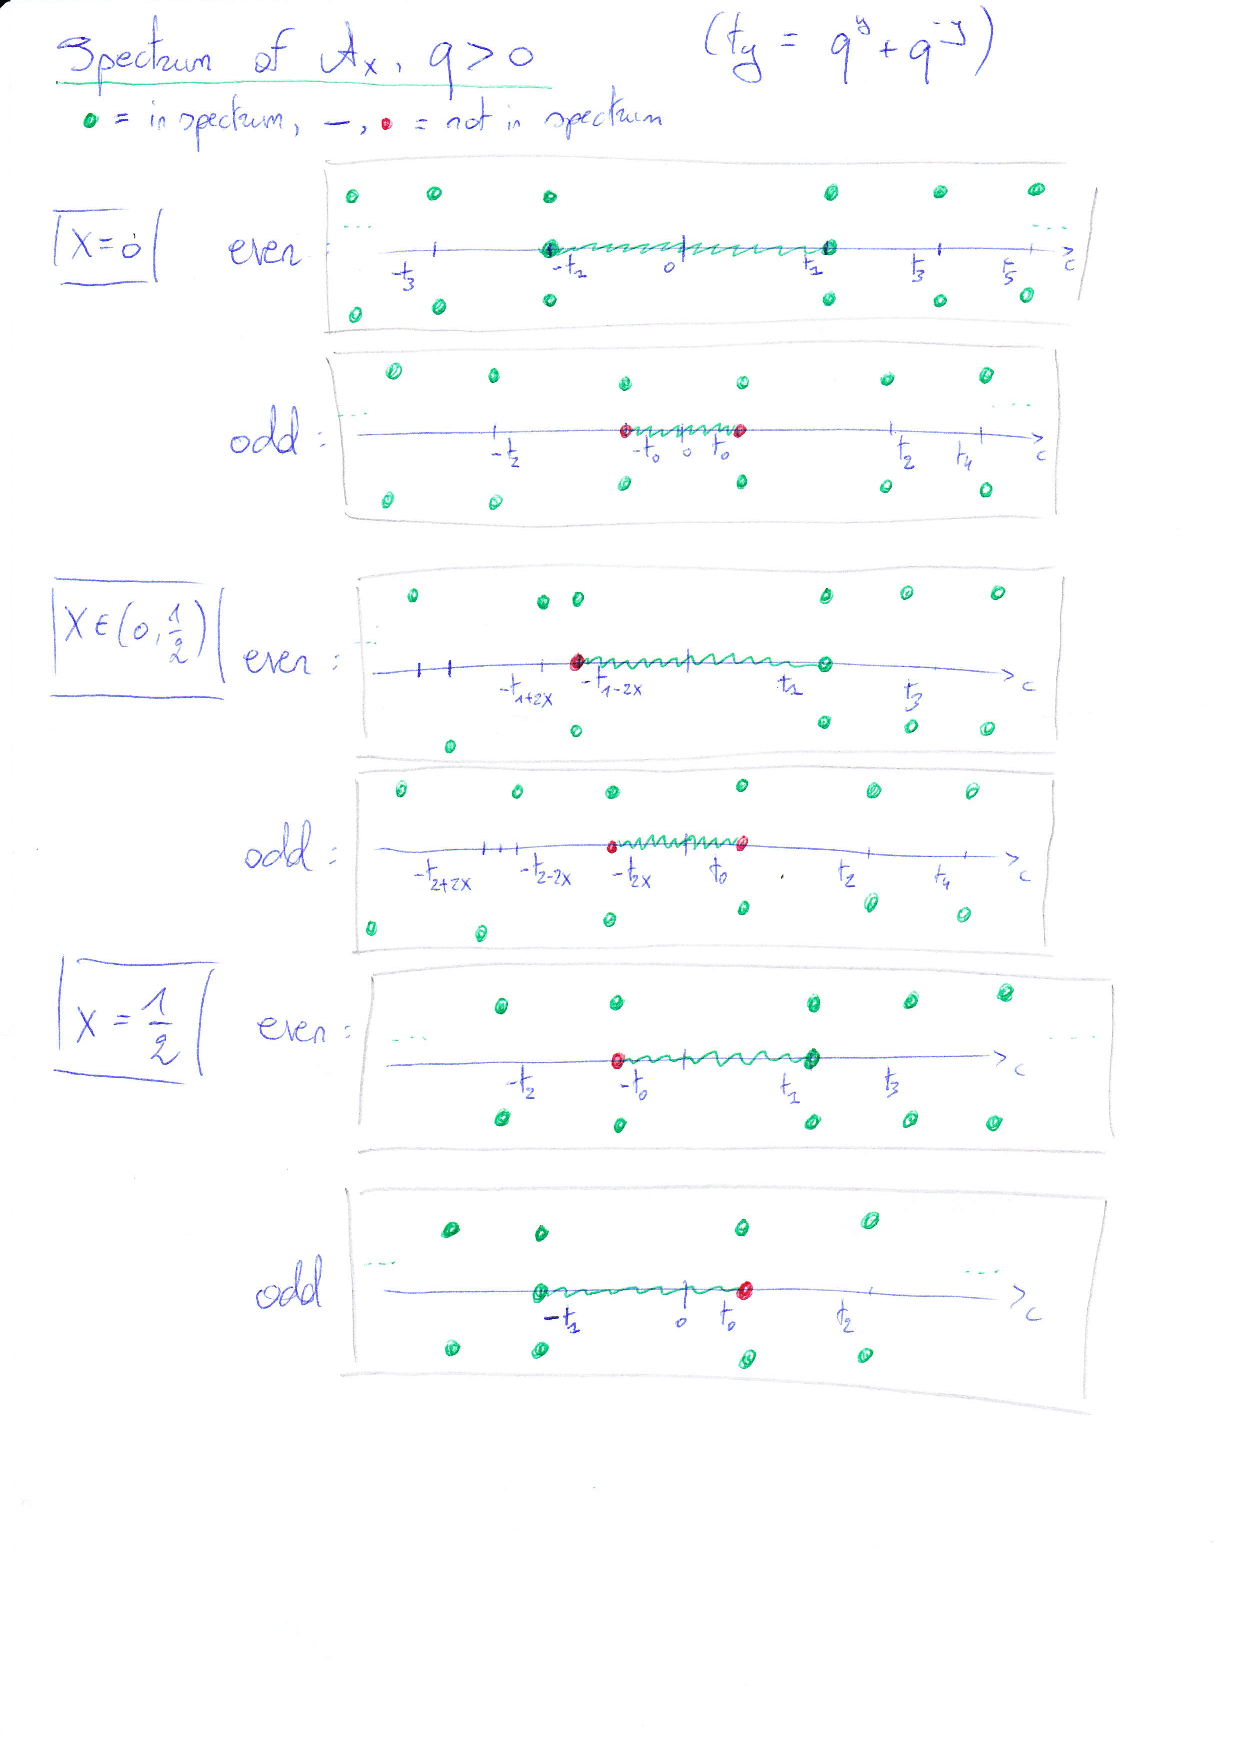
\includepdf[pages={1}]{ScanSpec.pdf}


% Make remark on regular representation cf. Koelink-Rosengren

% Include a concrete descripition of the universal envelope of $A_x$ from this?


%More generally, 

%As a concrete instance of the example of monoidal equivalence, let $\tilde{A}$ be the generalized compact Hopf face algebra obtained from the set $\tilde{I} =I_1\sqcup I_2$ with $I_1= \Z$ and $I_2= \{\bullet\}$ with the $B_{kl} =\emptyset$ and $E(k,l)$ for $k,l\neq \bullet$ as in section ..., with $B_{k,\bullet} = B_{\bullet,k}= \emptyset$, and $B_{\bullet,\bullet} = \{\pm\}$ with $E_{\bullet,\bullet} = \begin{pmatrix} 0 & |q|^{1/2} \\ -\sgn(q)|q|^{-1/2}&0\end{pmatrix}$ (with the basis ordered as $-,+$). Then this will be obtained from the direct sum of the functor from ... and the ordinary forgetful functor from $\Rep(SU_q(2))$ into $\Hilb$. It follows that the components $\tilde{A}(ij)$ can be described by the generators and relations as in ..., but with $F(\lambda)$ and $F(\rho)$ set equal to 1 whenever the corresponding index is $\bullet$.




% Study spectrum fundamental character
% Study dual quantum groupoid
% Make connection with dynamical cocycle
% In case of qgroupoid constructed from identity functor for Rep(SU_q(2)): rep theory of associated Galois object should just be: a single representation (Galois object is type I factor, cutdown of $B(\mathscr{L}^2(SU_q(2)))$). Yes: in general, Galois object is Morita equivalent with algebra of original ergodic action, should also be stressed for Podles spheres





%%% Local Variables: 
%%% mode: latex
%%% TeX-master: "dyn-suq-main"
%%% End: 
